\Echapter{Plotting Group FEAT Results Against Behavioral Measures}{Melissa A. Reilly}{mreilly@uw.edu}
\label{sec:groupfeatreport}
In neuroimaging research it is often beneficial to examine your results in conjunction with behavioral data to gain a more complete understanding of your effect. For example, it is certainly informative enough to look at group activation maps from subjects completing a memory task within the scanner; however, taking it a step further and incorporating the subjects' accuracy scores on the task arguably paints a richer picture. The example provided here does exactly this using a subset of a dataset from OpenFMRI.org  (\url{https://openfmri.org/dataset/ds000115}); these study subjects completed a memory task (the n-back) within the scanner and their accuracy scores were tracked. In this example, we will visualize each significant cluster, identify it, and plot its activation against the accuracy scores, all in the hopes of providing a clearer interpretation of the data.  
 
The code for this example is in \texttt{\$MAKEPIPELINES/WorkingMemory}. From within that directory, call the \texttt{PrepareExample} script to download the data and organize the directory - please note, this may take upwards of 30 minutes depending on your machine. 
\bashcmd{bash PrepareExample}

Once the download is complete, you can use the \texttt{"prepare"} target to run the lower-level FEATs.
\bashcmd{make -f makefiles/Makefile -k -j TARGET=prepare}

When the lower-level FEATs have completed, you can run the higher-level group analysis. A design file is already prepared for this:
\bashcmd{Feat lib/GROUP_2BACK.fsf}

If you open the file with Feat, you will note that the accuracy scores are already included (these scores were obtained from \texttt{data/demographics.txt}). You should check that the paths to the input files and standard brain are correct on your system. Once you have, click "Go" to run the analysis. 

This example uses a \texttt{makefile} in several smaller chunks to create the final product. The first part is to read the results from the \texttt{.gfeat} directory to generate masks for each significant cluster, and this utilizes \texttt{makefiles/Makefile.gfeat}. The second part is to use an FSL tool (\texttt{featquery}) to warp each mask into the subject's space and extract from it the mean z-score. We then use the \texttt{makefile} to create a spreadsheet within the \texttt{.gfeat} directory containing all the \texttt{featquery} z-scores, and finally, plot all those values against n-back performance and create an HTML report containing the plots as well as visualization of the clusters. Let's begin:
\begin{lstlisting}
	SHELL=/bin/bash
	export SHELL
	FSL_DIR=/usr/share/fsl/5.0
	
	ifeq "$(origin MAKEPIPELINES)" "undefined"
	MAKEPIPELINES=/project_space/makepipelines
	endif
	
	%*\lnote*group1: .readyforfq
	group2: FQresults_DATA
	group3: FQreport.html
	
	.PHONY: group1 featqueries group2 group3 clean.gfeat 
	
	clean.gfeat:
		rm -rf .readyforfq FQ* design2.mat sed* PLOTS MASKS CLUSTERS AQUERY .legend
		
	MYLOCAT=$(shell pwd)
	SCRIPTDIR=/project_space/makepipelines/WorkingMemoryIBIC/lib
	GF=$(basename $(shell basename `pwd`))
	ALLCOPES=$(wildcard cope*.feat)
	NUMMASKS=`ls MASKS | wc -l`
\end{lstlisting}
As you've seen before, we define our \texttt{SHELL} and \texttt{FSL_DIR} variables for consistency. We also include a "clean.gfeat" target to remove any of the outputs generated from this makefile. \lnum{1} \texttt{Makefile.gfeat} is run in several small chunks, so the \texttt{makefile} is divided into four phony targets to make this easier to run from the command line (three of the four are defined above, the forth is soon to come). Here we prepare some variables to help \maken{} complete the "group1" target, which creates the masks we need before we move into the subject directories. \texttt{MYLOCAT} is a variable to save our current location, and \texttt{GF} pulls the name of the .gfeat out of that. We define \texttt{SCRIPTDIR} to make a note of where we will be keeping some scripts we'll need later. The \texttt{ALLCOPES} variable complies a list of all the \texttt{cope*.feat} subdirectories within the \texttt{.gfeat}. The \texttt{NUMMASKS} variable will list all the masks in our soon-to-be-created \texttt{MASKS/} subdirectory. The "group1" target has only one prerequisite - \texttt{.readyforfq}.

\begin{lstlisting}
	.readyforfq:
		mkdir -p MASKS ;\
		mkdir -p CLUSTERS ;\
		
		%*\lnote*for COPE in $(ALLCOPES); do \
			%*\lnote*Zs=`ls $${COPE} | grep ^cluster_mask_zstat | wc -l` ;\
			WHICHZ=`seq 1 1 $${Zs}` ;\
			for CM in $${WHICHZ}; do \
			  %*\lnote*CNUM=`fslstats $${COPE}/cluster_mask_zstat$${CM}.nii.gz -R | awk '{ print $$2 }'` ;\
				for VAL in `seq -w 01 01 $${CNUM%%.*}`; do \
					$(FSL_DIR)/bin/fslmaths $${COPE}/cluster_mask_zstat$${CM}.nii.gz -thr $${VAL} -uthr $${VAL} -bin MASKS/$${COPE%.*}_z$${CM}_m$${VAL}.nii.gz ;\
					$(FSL_DIR)/bin/fslmaths $${COPE}/thresh_zstat$${CM}.nii.gz -mas MASKS/$${COPE%%.*}_z$${CM}_m$${VAL}.nii.gz CLUSTERS/$${COPE%.*}_z$${CM}_m$${VAL}.nii.gz ;\
				done ;\
			done ;\
		done ;\
		
		echo "$(NUMMASKS) masks found for $(GF)!";\
		touch .readyforfq
\end{lstlisting}

We begin by creating \texttt{MASKS/} and \texttt{CLUSTERS/} subdirectories to house the files we are about to create. We have already defined our \texttt{ALLCOPES} variable to be anything in the directory that fits the \texttt{cope*.feat} wildcard. In this example we have five copes, which are defined in \texttt{GROUP_2BACK/design.fsf}, but a given analysis could have any number, so a wildcard allows the program to be accommodating to both simpler and more complex designs. We want \maken{} to go into each of these copes ( \lnum{2}), find out how many \texttt{cluster_mask_zstat*.nii.gz} images are in each ( \lnum{3}), and then how many unique clusters are in each of those ( \lnum{4}). Though not ideal as far aesthetics are concerned, some shell variables and looping is the simplest way to do this.  (It is worth pointing out that the double \texttt{\$\$} is intentional -- when referring to shell variables \maken{} requires that you escape the \texttt{\$} with another \texttt{\$}.) For each unique cluster, \texttt{fslmaths} will create a binary mask to be placed in the \texttt{MASKS/} directory, and will then use that mask to create a thresholded image in the \texttt{CLUSTERS/} directory. The images are identical, except that the \texttt{MASKS/} one is binarized, and both are named according to the same convention (cope(\#)z(\#)m(\#).nii.gz). To put all this into practice, move into \texttt{GROUP_2BACK.gfeat} and run the "group1" target (NOTE: the "group1" target should NOT be parallelized):
\bashcmd{make -f ../makefiles/Makefile.gfeat -k group1}

As the "group1" target completes, it will print the number of masks created to the terminal. If there are no masks, there is nothing left to do; this analysis has 13 masks, which you can confirm by looking in the \texttt{MASKS/} subdirectory. The next step is to pass these masks to Featquery to run in the individual subject directories.

\begin{lstlisting}
	INTYPE=`cat design.fsf | grep "set fmri(inputtype)" | awk '{print $$$$3}'`
	INPUTS=$(shell cat `pwd`/design.fsf | grep "set feat_files" | awk '{print $$3}' | sed -e 's/"//g' | sed -e 's/\.feat.*/\.feat/')
	MASKLIST=$(basename $(basename $(shell ls MASKS)))
	
	%*\lnote*define query
	
	$(1)/fq_$(GF)_$(2)/report.txt: .readyforfq MASKS/$(2).nii.gz
		if [ $(INTYPE) -eq 1 ]; then COPENUM=`echo $(2) | cut -c 5-5`; else COPENUM=1; fi;\
		if [ -d $(1)/fq_$(GF)_$(2) ]; then rm -rf $(1)/fq_$(GF)_$(2)*; fi ;\
		$(FSL_DIR)/bin/featquery 1 $(1) 1 stats/zstat$$$${COPENUM} fq_$(GF)_$(2) $(MYLOCAT)/MASKS/$(2).nii.gz ;\
		echo "`cat $(1)/fq_$(GF)_$(2)/report.txt | awk '{print $$$$6}'`"
	
	endef
	
	%*\lnote*featqueries: $(foreach mask, $(MASKLIST), $(INPUTS:%=%/fq_$(GF)_$(mask)/report.txt))
	%*\lnote*$(foreach input,$(INPUTS),$(foreach mask,$(MASKLIST),$(eval $(call query,$(input),$(mask)))))
	
	clean.featqueries:
		rm -rfv $(foreach mask, $(MASKLIST), $(INPUTS:%=%/fq_$(GF)_$(mask)))
\end{lstlisting}

We will first define a few more variables to help us in running the \texttt{featqueries} target. The \texttt{INTYPE} variable reads the \texttt{.gfeat} design file to determine the input type: lower-level FEATs or cope images. We have already discussed that using shell variables requires an extra \texttt{\$}, but this gets even more complicated within a function. Additional escapes are necessary, hence the four \texttt{\$} in the \texttt{awk} command. The \texttt{INPUTS} variable reads the subject inputs from the design file, and uses some \texttt{sed} commands to remove some extensions and quotation marks. The \texttt{MASKLIST} variable is, of course, a list of all the masks contained in the \texttt{MASKS/} directory. Since a given group FEAT can have any number of masks, it is imperative that our program is flexible enough to deal with an unspecified number. We need to write a smarter recipe, where \maken{} will know to take each mask, run \texttt{featquery}, and create the output file -- and all this without us specifying how many masks or how they are named. \lnum{5} To do this, we define a function called \texttt{query}. The recipe defined within it is written like any other, but makes use of arguments, which appear as \texttt{\$(1)} and \texttt{\$(2)}. The intent is for \textbf{every} subject input (\texttt{\$(1)}) and for \textbf{every} mask we have generated (\texttt{\$(2)}), to run Featquery. Breaking down the recipe itself, the first line reads the \texttt{INTYPE} variable to determine how to define the \texttt{COPENUM} variable, as this is slightly different when using lower-level FEATs as inputs vs. cope images. The second line will check if a Featquery directory already exists for this subject and mask combination, and will delete it if it does. The third line actually runs the Featquery command.

\lnum{6} The phony "featqueries" target is defined using pattern substitution to be all the \texttt{report.txt} files that result from each featquery that is to be run. \lnum{7}We use a combination of \maken{}'s \texttt{foreach}, \texttt{eval}, and \texttt{call} to read all the masks contained in \texttt{MASKLIST} and all the subject inputs and submit each of those as arguments to \texttt{query}. We also define a "clean.featqueries" target to clean up all the Featquery outputs in the subject directories, which you may find useful for clutter-control after the spreadsheet has been generated. Run the "featqueries" target (and this time, parallelizing is encouraged!). 
\bashcmd{make -f ../makefiles/Makefile.gfeat -k -j featqueries}

When all the featqueries have completed, we are ready for the "group2" target:

\begin{lstlisting}
	RESULTS=$(MASKLIST:%=FQresults_%)
	INPUTNUM=`cat design.fsf | grep "set feat_files(" | wc -l`
\end{lstlisting}

There are only a few additional variables we need for completing the "group2" target, which compiles the spreadsheet (\texttt{FQresults_DATA}) containing the subject list, explanatory variables (EVs) and the mean values for each mask. \texttt{INPUTNUM} is a count of our subject inputs, which we are reading from the \texttt{design.fsf} file. \texttt{RESULTS} will hold the names of the files that will contain each column of the Featquery data in the spreadsheet.

\begin{lstlisting}	
	FQresults_DATA: .readyforfq FQresults_allSUBS FQresults_EVs $(RESULTS)
		paste -d',' FQresults_allSUBS FQresults_EVs $(RESULTS) > FQresults_DATA
\end{lstlisting}

\texttt{FQresults_DATA} will be a comma-separated spreadsheet that contains a column of the subject IDs, the names of the EVs and their values for each subject, and the names of the masks and the mean z-scores extracted from each of them for each subject. This file is created by pasting together several smaller files which are created below.

\begin{lstlisting}	
	FQresults_allSUBS: .readyforfq
		echo $(INPUTNUM)_SUBJECTS >> FQresults_allSUBS ;\
		echo $(INPUTS) >> FQresults_allSUBS ;\
		sed -i 's/ /\n/g' FQresults_allSUBS ;\
		rm -f sed*
\end{lstlisting}

\texttt{FQresults_allSUBS} is a text file containing each subject input. This file will be the first column of the \texttt{FQresults_DATA} spreadsheet. We simply print "\texttt{\$(INPUTNUM)_SUBJECTS}" to the file to serve as the column header. We \texttt{echo} the subject inputs (the contents of \texttt{\$(INPUTS)}) after that, and use \texttt{sed} to replace spaces with linebreaks. 

\begin{lstlisting}
	FQresults_EVs: .readyforfq
		NUMEV=`cat design.mat | awk '/NumWaves/ {print $$2}'` ;\
		%*\lnote*for EV in `seq 1 1 $${NUMEV}`; do \
			echo -ne "`cat design.fsf | grep "set fmri(evtitle$${EV})" | awk '{print $$3}'`," >> FQresults_EVs ;\
		done ;\
		echo >> FQresults_EVs ;\
		sed -i 's/"//g' FQresults_EVs ;\
		cat design.mat | tail -n $(INPUTNUM) >> design2.mat ;\
		NUMEV=`cat design.mat | awk '/NumWaves/ {print $$2}'` ;\
		sed -i 's/\t/,/g' design2.mat ;\
		cat design2.mat >> FQresults_EVs ;\
		sed -i 's/,$$//g' FQresults_EVs ;\
		sed -i 's/\"//g' FQresults_EVs ;\
		rm -f sed*
\end{lstlisting}

\texttt{FQresults_EVs} is another text file that will make up the column(s) immediately to the right of the subject inputs in \texttt{FQresults_DATA}, with the number of columns being determined by how many EVs were included in your \texttt{.gfeat} model (in our case, two). This recipe reads the \texttt{.gfeat}'s \texttt{design.mat} and \texttt{design.fsf} files, which contain all the information we need. Our end goal is to have a column for each EV where the EV name is printed in the first row and the value for each subject is printed on the subsequent lines, with each column being separated from the next with a comma. The \texttt{NUMEV} variable will read the header of the \texttt{design.mat} file to determine the number of EVs. \lnum{8} We will then use a simple \texttt{for loop} to read the names of the EVs one through \texttt{\$(NUMEV)} from \texttt{design.fsf}, and print all those names to the first row of \texttt{FQresults_EVs}. To obtain the values for these EVs, we essentially want the information contained in \texttt{design.mat} (but not all of it, and not in that format). We will copy the lines of \texttt{design.mat} that pertain to the individual subjects to \texttt{design2.mat} by using the \texttt{tail} command in conjunction with our \texttt{INPUTNUM} variable. A series of \texttt{sed} commands at the end of the recipe cleans up the data: the first exchanges tabs for commas, the second removes commas at the end of a line, and the last removes quotes that \texttt{FEAT} puts around the values. \texttt{FQresults_EVs} is now ready to be pasted next to \texttt{FQresults_allSUBs} in the creation of \texttt{FQresults_DATA}; we need only the columns that correspond to the individual clusters:
\begin{lstlisting}
	define getvalues
	
	FQresults_$(1): .readyforfq
		echo "$(1)" > temp_$(1) ;\
		for i in $(INPUTS); do echo `cat $$$${i}/fq_$(GF)_$(1)/report.txt | awk '{print $$$$6}'` >> temp_$(1); done ;\
		mv temp_$(1) FQresults_$(1)
		
	endef
	
	%*\lnote*$(foreach mask,$(MASKLIST),$(eval $(call getvalues,$(mask))))
\end{lstlisting}

As you well know by now, a function is our best bet for dealing with the unpredictable nature of the number of masks in our analysis. The \texttt{getvalues} function will create a text file for each mask called "\texttt{FQresults_MaskName}", which will have the name of the mask in the first row and the values for each subject in subsequent rows. \lnum{9}As we did with the \texttt{query} function, we submit each mask name as an argument. For each mask, the recipe looks into each subjects corresponding \texttt{featquery} results page, grabs the mean value, and prints it to the \texttt{FQresults} file for that mask.

Despite the lengthy explanation, this all runs very quickly. Run the "group2" target; you should not include a \texttt{-j} flag.
\bashcmd{make -f ../makefiles/Makefile.gfeat group2 -k}

Completion of the "group2" target yields a comma-separated spreadsheet that you can import to statistical or graphing software, but \maken{} still has a few more tricks up its sleeve. The "group3" target is by far the most impressive part of this example, so let's jump right in:

\begin{lstlisting}
	INTYPE2=`cat design.fsf | grep "set fmri(inputtype)" | awk '{print $$3}'`
	WHICHX=$(shell head -n 1 FQresults_EVs | awk -F ',' '{print $$NF}')
	PAGES=$(MASKLIST:%=AQUERY/%)
	STANDARD=/usr/share/fsl/5.0/data/standard/MNI152_T1_2mm_brain.nii.gz
\end{lstlisting}

We define just a few new variables to complete the "group3" target. The \texttt{INTYPE2} variable is similar to the \texttt{INTYPE} variable we defined earlier, different only in the number of escapes in the \texttt{awk} command, because we won't be using it within a function this time. When we call R to read \texttt{FQresults_DATA} and create the scatterplots, we need to specify which variable goes on the x-axis. For simplicity, it is assumed that the last EV entered is intended to be the x-axis variable, and thus \texttt{WHICHX} is defined to be the last item in the first row of \texttt{FQresults_EVs}. \texttt{PAGES} represents the names of the small chunks of HTML we will put together for each cluster we intend to display in our final report, which will be saved in a subdirectory called \texttt{AQUERY/}. \texttt{STANDARD} contains the full path to our standard brain, which should be modified to match your system.

\begin{lstlisting}
	Rplots: FQresults_DATA
		mkdir -p PLOTS ;\
		Rscript $(SCRIPTDIR)/AUTOPLOT.R $(WHICHX) FQresults_DATA $(shell pwd) ;\	
	
	define ssclust
	
	PLOTS/$(1)_brain.png: .readyforfq
		echo $(1) ;\
		mkdir -p PLOTS ;\
		/bin/bash $(SCRIPTDIR)/sscluster $(1) $(FSL_DIR) $(STANDARD)
			
	endef
	
	$(foreach cluster,$(MASKLIST),$(eval $(call ssclust,$(cluster))))
\end{lstlisting}

The phony "Rplots" target will create a directory to house some of the images we're about to create, and will call the R script (located in the \texttt{lib/} directory) to create the scatterplots. Each plot will be saved according to the mask name.  Within the \texttt{ssclust} function we will call an external script to create a screenshot of each cluster to view alongside the corresponding scatterplot, saved as \texttt{PLOTS/MaskName_brain.png}. These screenshots will overlay the cluster on the specified standard brain, and will capture ten images in each plane to create a visual representation of each cluster.

\begin{lstlisting}
	define atlasquery
	
	AQUERY/$(1): .readyforfq $(MASKLIST:%=PLOTS/%_brain.png) Rplots .legend
		mkdir -p AQUERY ;\
		HTML=AQUERY/$(1) ;\
		echo "<img src="PLOTS/$(1).png" alt="$(1).png">" >> $$$${HTML} ;\
		echo "<img src="PLOTS/$(1)_brain.png" alt="$(1)_brain.png" width="60%">" >> $$$${HTML} ;\
		echo "<br><br><table width="100%"><tr>" >> $$$${HTML} ;\
		HOCORT=`$(FSL_DIR)/bin/atlasquery -a "Harvard-Oxford Cortical Structural Atlas (Lateralized)" -m CLUSTERS/$(1)` ;\
		echo "<td valign="top"><p align="left">Harvard-Oxford Cortical Structural Atlas:<br><small>`echo $$$${HOCORT} | sed -e 's/[0-9] /<br>/g'`</small></p></td>" >> $$$${HTML} ;\
		HOSUBCORT=`$(FSL_DIR)/bin/atlasquery -a "Harvard-Oxford Subcortical Structural Atlas" -m CLUSTERS/$(1)` ;\
		echo "<td valign="top"><p align="left">Harvard-Oxford Subcortical Structural Atlas:<br><small>`echo $$$${HOSUBCORT} | sed -e 's/[0-9] /<br>/g'`</small></p></td>" >> $$$${HTML} ;\
		CEREBELL=`$(FSL_DIR)/bin/atlasquery -a "Cerebellar Atlas in MNI152 space after normalization with FLIRT" -m CLUSTERS/$(1)` ;\
		echo "<td valign="top"><p align="left">Cerebellar Atlas after normalization with FLIRT:<br><small>`echo $$$${CEREBELL} | sed -e 's/[0-9] /<br>/g'`</small></p></td>" >> $$$${HTML} ;\
		JUEL=`$(FSL_DIR)/bin/atlasquery -a "Juelich Histological Atlas" -m CLUSTERS/$(1)` ;\
		echo "<td valign="top"><p align="left">Juelich Histological Atlas:<br><small>`echo $$$${JUEL} | sed -e 's/[0-9] /<br>/g'`</small></p></td>" >> $$$${HTML} ;\
		echo "</tr></table>" >> $$$${HTML} ;\
		echo "<p>- - - - - - - - - - - - - - - - - - - - -</p>" >> $$$${HTML}
				
	endef
	
	$(foreach cluster,$(MASKLIST),$(eval $(call atlasquery,$(cluster))))
\end{lstlisting}

The final \texttt{FQreport.html} file is built from a number of smaller pieces, and the \texttt{atlasquery} function will create most of these pieces. We first create a \texttt{AQUERY/} subdirectory to put all these pieces in, where "AQUERY" is short for \texttt{atlasquery}, an FSL tool that gives the average probability of a mask being a member of the different labeled regions of a given atlas. The small pieces of HTML we are compiling here will, for all of our masks, place the scatterplot next to the corresponding cluster screenshot, and below that, will provide the \texttt{atlasquery} outputs for four different atlases: the Juelich Histological Atlas, Cerebellar Atlas in MNI152 space after normalization with FLIRT, and the Harvard-Oxford Cortical and Subcortical Structural Atlases. These individual pieces can be viewed on their own, but we will pull them all together to create the \texttt{FQreport.html} file:

\begin{lstlisting}
	FQreport.html: $(MASKLIST:%=AQUERY/%)
		REPORT=FQreport.html ;\
		echo "<!DOCTYPE html><html>" > $${REPORT} ;\
		echo "<head>" >> $${REPORT} ;\
		echo "<title>$(GF).gfeat</title>" >> $${REPORT} ;\
		echo "</head>" >> $${REPORT} ;\
		echo "<body bgcolor="#000000"><font face="Arial" color="#ffffff">" >> $${REPORT} ;\
		echo "<center>" >> $${REPORT} ;\
		echo "<p>Scatter plots depicting the relationship between brain activity and behavioral measures are provided for descriptive purposes only</p>" >> $${REPORT} ;\
		%*\lnote*for page in $(PAGES); do echo "<BR><BR>">> $${REPORT}; cat $${page} >> $${REPORT}; done ;\
		echo "</center></body></html>" >> $${REPORT}
\end{lstlisting}

The last bit of code here serves as a template for the HTML report. It contains code pertaining to basic styling and formatting of the HTML document, and \lnum{10} then looks to \texttt{\$(PAGES)} to get the names of the HTML pieces contained in the \texttt{AQUERY/} subdirectory, and embeds those into this report. To run this final bit, you should feel free to parallelize:
\bashcmd{make -f ../makefiles/Makefile.gfeat group3 -k -j}

An example of the final report is shown below (for a clearer view, a pre-generated copy is saved at \texttt{lib/pregenREPORT.html}; it provides a clear description of the data, and together with the \texttt{FQresults_DATA} file, provides an excellent stepping stone for further analysis.

\begin{figure}
	\begin{center}
          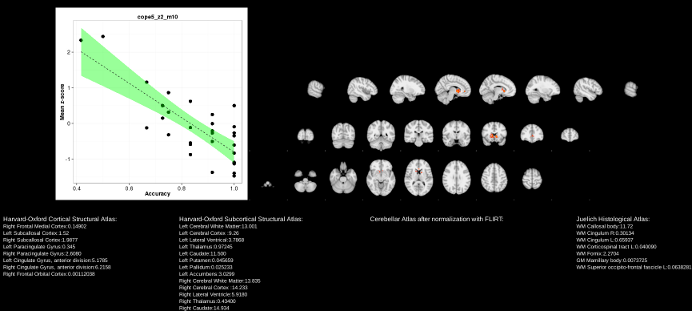
\includegraphics[scale=.6]{../images/SSreport.png}
		\caption{Report plotting group FEAT results against behavioral measures.}
                \label{fig:fqresults}
	\end{center}
\end{figure}
